\chapter{Sediment transport}
\label{chap:Transporte-Sedimentos}
%    O transporte de sedimentos é o movimento de partículas sólidas, carregadas por um fluido em uma certa distância, que escoam na mesma direção. O transporte é uma combinação entre a ação da gravidade no sistema e as forças de arraste do fluido. Um vasto número de fenômenos estão relacionados com o transporte de fluidos, como em processos industriais (ao transportar minérios por um mineroduto), ou a transformação das paisagens (na formação ou desaparecimento de dunas) \cite{Granular_Media_Between_Fluid_and_Solid}. O resultado de ação dos diferentes tipos de fluidos, com características diversas, resultam em fenômenos diferentes, como processos causados por água: erosão pluvial, erosão fluvial e assoreamento; e processos causados pelo vento: dunas, desertificação.

    The sediment transport is the movement of solid particles, carried by a fluid over a distance, flowing in the same direction. The transport is a combination of action of gravity on the system and the fluid forces, mainly the fluid drag force. A vast number of phenomena are related to the fluid transport, such as in industrial processes (when transporting ores through a pipeline), or the transformation of landscapes (in the formation or disappearance of dunes) \cite{Granular_Media_Between_Fluid_and_Solid}. The different fluids acts differently, resulting in phenomena like: pluvial erosion, river erosion and silting, all caused by water; and phenomena caused by wind, like dunes and desertification. 

%    Pode-se classificar os tipos de transporte como mostrado na figura \ref{fig:transport_mode}, em que os sedimentos são retirados de um local e depositados em outro, em diferentes escalas temporais e espaciais. Uma formação pode aparecer na escala de minutos com alguns centímetros de altura nos fundos de rios e oceanos, até formações geológicas de milhares de anos com centenas de quilômetros de extensão.

    The types of transport can be classified as shown in figure \ref{fig:transport_mode}, in which sediments are removed from one location and deposited in another, in different temporal and spatial scales. A formation can appear on the scale of minutes from a few centimetres high on the bottoms of rivers and oceans, to geological formations thousands of years old and hundreds of kilometres long.

\begin{figure}
    \centering
    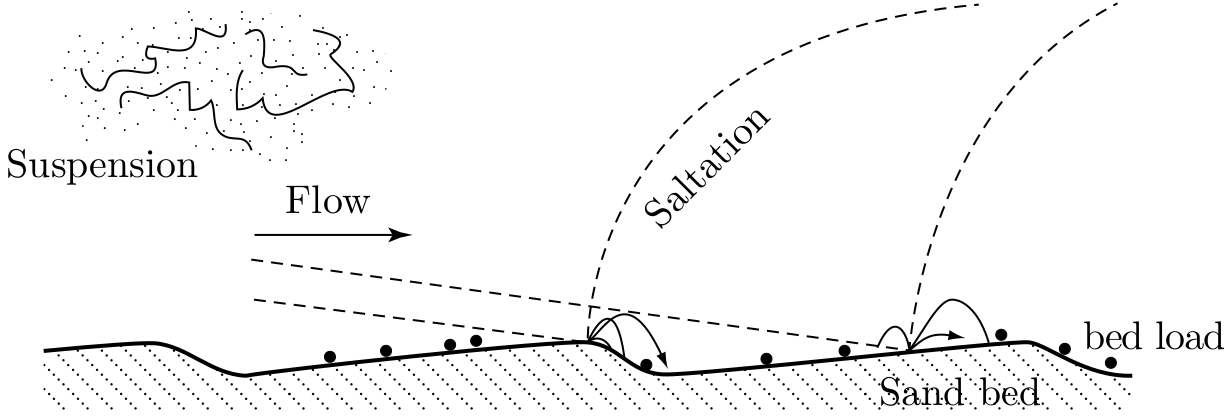
\includegraphics[width = 0.75 \textwidth]{04-figuras/TransportModes.png}
    \caption[Transport modes.]{Schematic diagram of different transport modes. Figure taken from \cite{Granular_Media_Between_Fluid_and_Solid}.}
    \label{fig:transport_mode}
\end{figure}

%    Materiais sólidos podem ser transportados pelos seguintes modos: \textit{bed load}, que é o transporte de material rolando sobre uma fina camada da base granular e ocorre quando a força gravitacional é a força mais preponderante no sistema \cite{Bedforms_in_a_turbulent_stream} ocorrer no fundo dos riachos e lagos e na superfície de um terreno; \textit{saltation}, que é o transporte de material que colide com a base granular em saltos, ocorrendo quando as forças gravitacionais e de arraste são as mais relevantes no sistema, podendo ser visto em rios e nos processos erosivos dos ventos; e finalmente \textit{suspension}, que é o modo de transporte de material em que as forças de arraste causadas pelas flutuações turbulentas passam a ser da ordem de grandeza do peso dos grãos e dominam a dinâmica do sistema \cite{FVSCS}, podendo ser observado em tempestades de areia ou ao varrer-se a poeira de casa.

    Solid materials can be transported by the following modes: bedload, which is the transport of material rolling over a thin layer of the granular base and occurs when the gravitational force is the most prevalent force in the system \cite{Bedforms_in_a_turbulent_stream}. Bedload can occur on the bottom of streams and lakes and on the surface of a land. Saltation is the transport mode of materials that collides with the granular base in jumps, occurring when gravitational and drag forces are the most relevant in the system, and can be seen in rivers and in wind erosive processes. Finally suspension is the transport mode of materials in which the drag forces caused by turbulent fluctuations become the order of magnitude of the grain weight and dominate the dynamics of the system \cite{FVSCS}. Suspension may be observed in sandstorms or when sweeping house dust. 

%    Modelos monofásicos não são capazes de reproduzir a física envolvida neste problema. Modelos de materiais granulares sem a presença de fluido não exibem as propriedades dos modos de transporte como \textit{bed load}, \textit{saltation} e \textit{suspension}. Assim como os modelos de fluidos sem os sedimentos não são capazes de descrever as propriedades de deposição, de erosão ou mesmo de saturação. Sendo assim, é necessário que o modelo possua as duas fases estejam descritas, sedimento e fluido.

    Single-phase models are not able to reproduce the physics involved in this problem. Models of granular materials without the presence of fluid do not exhibit the properties of transport modes such as bedload, saltation and suspension. Likewise, fluid models without sediments are not able to describe the deposition, erosion or even saturation properties. Therefore, it is necessary that the model has the two phases described, sediment and fluid. 

%    Duas propriedades intrínsecas do arraste são a escala de comprimento de saturação $L_{sat}$ e a escala de tempo de saturação $T_{sat}$. A escala de comprimento de saturação quantifica a distância característica para que os grãos tenham a densidade máxima transportada pelo fluido $q_{sat}$. Já a escala de tempo de saturação indica o tempo característico para que a densidade de material transportado decaia quando a velocidade do fluido decair bruscamente, ou para que a densidade de material transportado aumente quando a velocidade do fluido aumentar bruscamente \cite{Granular_Media_Between_Fluid_and_Solid}.

    Two intrinsic properties of drag are the saturation length scale $L_\textrm{sat}$ and the saturation time scale $T_\textrm{sat}$. The saturation length scale quantifies the characteristic distance for the grains to have the maximum density transported by the fluid $q_\textrm{sat}$. The saturation time scale, on the other hand, indicates the characteristic time for the transported material density to decay when the fluid velocity decreases sharply, or for the transported material density to increase when the fluid velocity increases sharply \cite{Granular_Media_Between_Fluid_and_Solid}. The main transport governing equation is the Transport Equation, which relates the quantities:
\begin{equation}
    T_\textrm{sat} \frac{\partial q}{\partial t} + L_\textrm{sat} \frac{\partial q}{\partial x} = q_\textrm{sat} - q,
    \label{equ:transporte}
\end{equation}
where $T_{sat}$ is the saturation time that flux takes to adjust, $L_{sat}$ is the saturation length that flux takes to adjust, $q_{sat}$ is the saturated flux, $q$ is the flux, $t$ is the time and $x$ is the direction of the flux.

%    Visando um modelo que seja capaz de reproduzir tais características, o uso de \textit{Discrete Element Method (DEM)} combinado com o uso de \textit{Finite Element Method (FEM)} simulam o comportamento dos materiais e do fluido, interagindo as diferentes abordagens contínua do fluido e discreta do material granular.

    Aiming at a model capable of reproducing such characteristics, the use of DEM combined with the use of FDM simulate the behavior of grains and fluid, interacting with different approaches to continuous fluid and discrete to granular material. 

%    Para descrever o comportamento interativo entre o fluido e o material granular, utilizaremos simulações computacionais baseadas nos trabalhos do Dr. Philippe Claudin \cite{Numerical_simulation_of_turbulent_sediment_transport, Sand_ripples_and_dunes, Direct_numerical_simulations_of_aeolian_sand_ripples}. Impondo as condições iniciais do fluido, mede-se o tempo necessário para que o novo regime atinja as condições estacionárias. O número de grãos que escoa pelo sistema, no regime estacionário, fornece o fluxo volumétrico saturado $q_{sat}$, que serve de parâmetro para comparação e medição do tempo de saturação e do comprimento de saturação. Repete-se o processo para cada parâmetro de entrada, quantificando assim, as diferentes transições entre os modos de transporte.

    To describe the interactive behavior between fluid and granular material, we will use computer simulations based on the work of Dr. Philippe Claudin \cite{Numerical_simulation_of_turbulent_sediment_transport, Sand_ripples_and_dunes, Direct_numerical_simulations_of_aeolian_sand_ripples}. By imposing the initial conditions of the fluid, the time needed for the new regime to reach stationary conditions is measured. The number of grains flowing through the system, in the steady state, provides the saturated volumetric flow $q_\textrm{sat}$, which serves as a parameter for comparing and measuring the saturation time and the saturation length. The process is repeated for each input parameter, thus quantifying the different transitions between modes of transport.

%    Inicialmente, validamos o fluido, e então, interagimos fluido e grãos. Na validação do fluido observamos se a discretização contempla o modelo contínuo. Montamos uma malha unidimensional espaçada por um tamanho fixo ao longo de uma reta, que denominamos de direção $y$. A ideia é que haja escoamento na direção perpendicular, denominada de $x$, e que as camadas não troquem massa ou pressão, mas quantidade de movimento, que se reflete na velocidade do fluido. Tensão de cisalhamento e velocidade do fluido estão intimamente associados pelo conjunto de equações \ref{equ:fluido_x} e \ref{equ:cisalhamento}.

%    Considerando que o cisalhamento do fluido pode ser predominantemente laminar, ou seja, quando o número de Reynolds (equação \ref{equ:Reynolds}) for muito pequeno (tipicamente $\mathcal{R}<0.01$), o fluido escoará em regime laminar. Podemos aproximar o cisalhamento por contribuição apenas da parcela de viscosidade do fluido, e teremos então uma equação do tipo difusão linear, e que possui solução analítica no regime estacionário dada pela equação \ref{equ:fluido_laminar}:
%\begin{equation}
%    \label{equ:fluido_laminar}
%    u(y) = \frac{u_{*}^{2}}{\nu}y,
%\end{equation}
%em que $u$ é a velocidade de escoamento do fluido, $u_{*}$ é a velocidade característica de cisalhamento imposta ao fluido, $\nu$ é a viscosidade do fluido e $y$ é a altura da coluna de fluido.

%\begin{equation}
%    \label{equ:fluido_laminar_tempo}
%    \begin{aligned}
%        u(y,t) & = (u^{top}-u^{bottom})\frac{y}{l} +u^{top} +\sum_{n=1}^{\infty} {c_{n} e^{-\left(\frac{n\pi\alpha}{l}\right)^{2}t}sin\left(\frac{n\pi y}{l}\right)} \\
%        c_{n} & = \frac{2}{l} \int_{0}^{l} {\left[f(y) -(u^{top}-u^{bottom})\frac{y}{l} -u^{bottom}\right] sin\left(\frac{n\pi y}{l}\right)} dy,
%    \end{aligned}
%\end{equation}
%em que $u$ é a velocidade de escoamento do fluido na direção $x$ em função da altura $y$ e do tempo $t$, $u^{top}$ é a velocidade do fluido na fronteira superior do sistema, $u^{bottom}$ é a velocidade do fluido na fronteira inferior do sistema e é nula, $c_{n}$ são os coeficientes de Fourier, $l$ é a altura do sistema, $\alpha$ é o coeficiente da difusão que se relaciona com a densidade $\rho$ e com a viscosidade $\nu$.

%    Considerando que o cisalhamento do fluido pode ser predominantemente turbulento, ou seja, quando o número de Reynolds (equação \ref{equ:Reynolds}) for muito grande (tipicamente $\mathcal{R}>1000$), o fluido escoará em regime turbulento. Podemos aproximar o cisalhamento por contribuição apenas da parcela de viscosidade turbulenta, e teremos então o regime estacionário dado pela equação \ref{equ:fluido_turbulento}.

%\begin{equation}
%    \label{equ:fluido_turbulento}
%    u(y) = \frac{u_{*}}{\kappa} ln\left|1+\frac{u_{*}}{0,1\nu}y\right|,
%\end{equation}
%em que $u$ é a velocidade de escoamento do fluido, $u_{*}$ é a velocidade característica de cisalhamento imposta ao fluido, $\nu$ é a viscosidade do fluido, $\kappa \simeq 0,4$ é a constante de von Karman e $y$ é a altura da coluna de fluido \cite{Numerical_simulation_of_turbulent_sediment_transport}.

%    Para descobrir o regime estacionário do fluido, utilizamos o método de Runge-Kutta de 4ª ordem sobre a equação \ref{equ:fluido_estacionario}, que é a equação de van Driest \cite{Numerical_simulation_of_turbulent_sediment_transport}, e encontramos a curva da figura \ref{fig:RK}.

%\begin{equation}
%    \label{equ:fluido_estacionario}
%    \left(\nu+l^{2}\left|\frac{\partial u}{\partial y}\right|\right)\frac{\partial u}{\partial y} = u_{*}^{2},
%\end{equation}
%em que $\nu$ é a viscosidade do sistema, $u$ é a velocidade de escoamento do fluido, $u_{*}$ é a velocidade característica do cisalhamento imposto ao fluido e $l$ é o comprimento de mistura da turbulência, dado pela equação \ref{equ:comprimento_turbulencia_fluido}.

%\begin{figure}
%    \centering
%    \begin{minipage}{.45\linewidth}
%        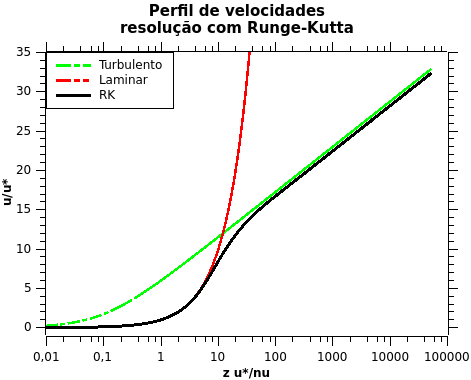
\includegraphics[width = 0.9\textwidth]{04-figuras/Velocidade_Fluido_RK.png}
%        \subcaption{Velocidade}
%        \label{fig:Velocidade_RK}
%    \end{minipage}
%    \begin{minipage}{.45\linewidth}
%        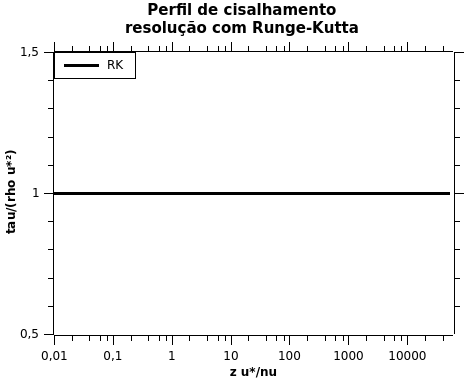
\includegraphics[width = 0.9\textwidth]{04-figuras/Cisalhamento_Fluido_RK.png}
%        \subcaption{Cisalhamento}
%        \label{fig:Cisalhamento_RK}
%    \end{minipage}
%    \caption{Resultado do fluido estacionário. Na figura \ref{fig:Velocidade_RK} está a solução da equação \ref{equ:fluido_estacionario} para a velocidade, utilizando o método de Runge-Kutta de 4ª ordem. Na figura \ref{fig:Cisalhamento_RK} está a solução do cisalhamento.}
%    \label{fig:RK}
%\end{figure}

%    As simulações do fluido colapsam em uma única curva com diferentes valores do número de Reynolds. A figura \ref{fig:Simulacao_Fluido} contém os perfis de velocidade normalizados para diferentes números de Reynolds. A validação das simulações é obtida por meio da comparação entre o cisalhamento do fluido no regime estacionário e o esperado nas equações do cisalhamento, em regime estacionário. Apesar da velocidade apresentar um perfil não linear por inserção da turbulência, observamos que o cisalhamento é constante ao longo do perfil de alturas. Com a constância do cisalhamento, tem-se a indicação de que o sistema é invariante no tempo, e portanto está no regime estacionário.

%\begin{figure}
%    \centering
%    \begin{minipage}{.45\linewidth}
%        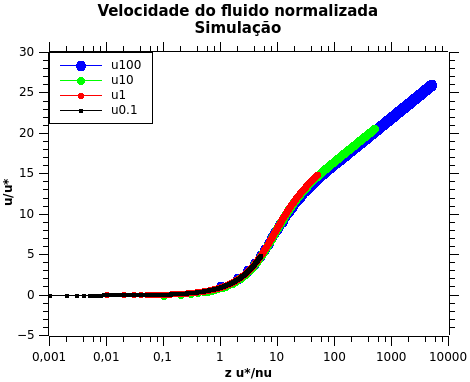
\includegraphics[width = 0.9\textwidth]{04-figuras/Velocidade_Fluido_Simulacao.png}
%        \subcaption{Velocidade}
%        \label{fig:Velocidade_Fluido}
%    \end{minipage}
%    \begin{minipage}{.45\linewidth}
%        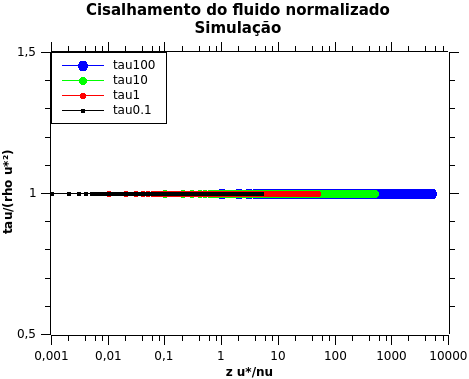
\includegraphics[width = 0.9\textwidth]{04-figuras/Cisalhamento_Fluido_Simulacao.png}
%        \subcaption{Cisalhamento}
%        \label{fig:Cisalhamento_Fluido}
%    \end{minipage}
%    \caption{Resultado do fluido estacionário. Na figura \ref{fig:Velocidade_Fluido} está a evolução do conjunto de equações \ref{equ:fluido_x} e \ref{equ:cisalhamento} com a observação da velocidade. Na figura \ref{fig:Cisalhamento_Fluido} está o cisalhamento. Em ambos os casos, há variação do número de Reynolds para cada uma das curvas.}
%    \label{fig:Simulacao_Fluido}
%\end{figure}

%    Comparando os perfis do método de Runge-Kutta de 4ª ordem para resolver as equações \ref{equ:fluido_laminar}, \ref{equ:fluido_turbulento} e \ref{equ:fluido_estacionario}, vimos na figura \ref{fig:Velocidade_RK} que o perfil laminar encaixa-se para números de Reynolds baixos e que o perfil turbulento encaixa-se em números de Reynolds altos. Por se tratar do regime estacionário, o perfil de cisalhamento é uma constante, como na figura \ref{fig:Cisalhamento_RK}.

%    Após checado que as simulações do fluido convergem para a solução apresentada pelo Runge-Kutta de 4ª ordem, apresentado na figura \ref{fig:Velocidade_Fluido}, e que o perfil de cisalhamento do fluido é constante ao longo de toda altura, apresentado na figura \ref{fig:Cisalhamento_Fluido}, inserimos os grãos no sistema e verificamos se as propriedades ainda continuam válidas.

%    A figura \ref{fig:Fluido_Grao} mostra o cisalhamento de um sistema com $8000$ grãos, com dispersão dos diâmetros em $20\%$, constante de mola na direção normal $k_{n} = 1000$, constante de mola na direção tangencial $k_{t} = 750$, coeficiente de amortecimento $\gamma = 13,6265$, coeficiente de atrito $\mu = 0,5$, distribuídos em uma base de $200$ diâmetros de grão, com condição periódica de contorno, imersos em um fluido de razão de densidade $1/2$, número de Reynolds $\mathcal{R} = 0.1$ e número de Shields $\Theta = 0.01$. O resultado é amostrado em $20$ simulações, com o cálculo de tensão de cisalhamento nos grãos descrito pela equação \ref{equ:Cisalhamento_Graos} \cite{Granular_Physics, Mechanical_properties_of_inclined_frictional_granular_layers}:
%\begin{equation}
%    \label{equ:Cisalhamento_Graos}
%    \sigma_{xy} = \sum_{i} \sum_{j} \frac{\vec{F}_{i,j}.\hat{x} \vec{r}_{i,j}.\hat{y}}{2d\sqrt{\pi}} \int_{0}^{1} e^{-{\frac{y-r_{i}.\hat{y}-r_{i,j}.\hat{y}s}{w}}^{2}} \mathrm{d}s,
%\end{equation}
%em que $\sigma_{xy}$ é o perfil de cisalhamento que os grãos sofrem, $i$ e $j$ são os índices dos grãos que estão em contato, $\vec{F}_{i,j}.\hat{x}$ é a componente $x$ da força de contato entre os grãos, $\vec{r}_{i,j}.\hat{y}$ é a componente do vetor de contato entre os grãos, $d$ é o diâmetro médio dos grãos, $y$ é a altura do perfil analisado, $r_{i}.\hat{y}$ é a posição do grão e a integral é uma função de \textit{coarse-graining}, que deve ser positiva e normalizada. Neste caso escolhemos a função gaussiana para melhor suavização do perfil de cisalhamento.

%\begin{figure}
%    \centering
%    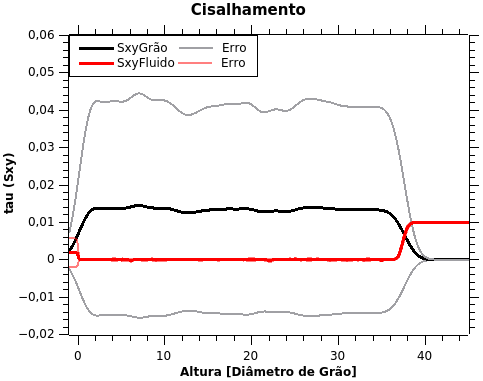
\includegraphics[width = 0.45\textwidth]{04-figuras/Cisalhamento_Fluido_Grao.png}
%    \caption{Perfil de cisalhamento dos grãos e do fluido no regime estacionário.}
%    \label{fig:Fluido_Grao}
%\end{figure}

%    Para o sistema da figura \ref{fig:Fluido_Grao} escolhemos os parâmetros do número de Shields e de Reynolds que não arrastassem os grãos, para podermos analisar a influência do fluido no regime estacionário. O perfil de cisalhamento transmitido do fluido para os grãos encaixa-se dentro da faixa esperada, apesar dos cisalhamentos não serem os mesmo, a convergência não é exata por se tratar da interação do meio contínuo com o meio discreto.

%    Até agora, estivemos preocupados com a consistência física do problema. Os próximos passo são reproduzir os modos de transportes \textit{bead load} e \textit{saltation} descritos por Orencio Durán \cite{Numerical_simulation_of_turbulent_sediment_transport} e medir os tempos de para a acomodação do regime estacionário, determinando assim o tempo de saturação dos modos de transporte dos sedimentos.

\begin{figure}
    \centering
    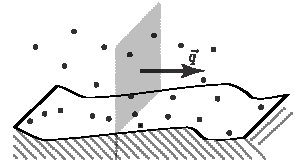
\includegraphics[width=0.65\textwidth]{04-figuras/flux_density.pdf}
    \caption[Transport volumetric flux.]{A schematic of the volumetric flux $q$. Figure taken from \cite{Granular_Media_Between_Fluid_and_Solid}.}
    \label{fig:flux_density}
\end{figure}

    The saturated flux $q_\textrm{sat}$ is the main quantity we analyse the sediment transport. It measures the volume of the particles crossing a vertical surface of unit transverse size per unit time. The definition is as it follows:
\begin{equation}
    q_\textrm{sat} = \frac{1}{A \phi_b} \frac{\pi}{6}d^3 \sum_p u^p,
    \label{equ:qsat}
\end{equation}
where $A$ is the surface area that particles cross, $\phi_b$ is the packing fraction of the base, $d$ is the average grain diameter and $u^p$ is the grain velocity.

    Other two quantities related to the saturated flux is the number of of transported grains per unit area $n$ and the mean grain horizontal velocity $u^p$:
\begin{equation}
    n = \frac{\left(\sum_p u^p\right)^2}{A\sum_p {u^p}^2}
    \label{equ:n}
\end{equation}
\begin{equation}
    \bar{u}^p = \sum_p \frac{\sum_p {u^p}^2}{\sum_p {u^p}}
    \label{equ:up}
\end{equation}
and the relation between $q_\textrm{sat}$, $n$ and $\bar{u}^p$ is:
\begin{equation}
    q_\textrm{sat} = \frac{1}{\phi_b} \frac{\pi}{6} d^3 n \bar{u}^p.
\end{equation}

\section{Threshold}
    To describe the bedload transportation threshold, we are going to use the same idea from the Book \cite{Granular_Media_Between_Fluid_and_Solid}. It consists in writing momentum equations in steady state ($\sum F = 0$) and find the values where they get balanced, for the maximum velocity of the fluid lays the grains in rest. So, the forces that will hold grains statically until moving are given by:
\begin{equation}
    m\frac{\partial u_p}{\partial t} = F_{Drag} + F_{Friction},
\end{equation}
where the acceleration of the particle is $m\frac{\partial u_p}{\partial t} = 0$, due to the steady state regime, $F_{Drag}$ is the drag force, $F_{Friction}$ is the friction force.

\begin{equation}
    F_{Drag} = 3\pi \rho_f \nu d\left(u_f-u_p\right),
\end{equation}
is the drag force onto grains, where $\rho_f$ is the density of the fluid, $\nu$ is the viscosity of the fluid, $d$ is the diameter of the grain, $u_f$ is the fluid velocity and $u_p$ is the grains velocity.

\begin{equation}
    F_{Friction} = -\mu_s F_{Gravity},
\end{equation}
is the friction force, and is dependent of the gravity, where $\mu_s$ is the static friction coefficient, related to the Coulomb friction.

\begin{equation}
    F_{Gravity} = \frac{\pi}{6}d^3\left(\rho_p-\rho_f\right)g,
\end{equation}
is the gravity force onto the grains, where $\rho_p$ is the grains density and $g$ is the gravitational acceleration.

    And since we know that the fluid shear stress is given by:
\begin{equation}
    \tau_f = \rho_f \nu \frac{\partial u_f}{\partial z},
\end{equation}
where $\tau_f$ is the fluid shear stress, these equations combined and considering the fact that only the upper half of the particle feels drag force, we have:
\begin{equation}
    u_f = \frac{\tau_f}{\rho_f\nu}\frac{d}{2}.
\end{equation}
while $u_p = 0$.

    Using the Shields number (Equation \ref{equ:Shields}) and manipulating previous equations, when applied drag force is equals to friction force, we can find the threshold by:
\begin{equation}
    \Theta_{Th} = \frac{2}{9}\mu_s.
\end{equation} 

\section{Contribution of moving grains}
    To introduce the contribution of the moving grains, we are still going to use most of the previous calculation. Still, particles have reached steady state, so $m\frac{\partial u_p}{\partial t} = 0$ is still valid. Considering that grains are moving, we have the balance force:
\begin{equation}
    0 = F_{Drag} + F_{Friction} + F_{Grains},
\end{equation}
now $F_{Grains}$ is the force due to the moving grains, where it is:
\begin{equation}
    F_{Grains} = \frac{\rho_p d^3 u_p \tau_p d^2}{d^2/\nu},
\end{equation}
where $\rho_p d^3 u_p$ is the momentum carried by moving grains, $\tau_p$ is the grains shear stress and $d^2/\nu$ is the characteristic time to this viscous contact dynamics.

    Looking to the limit just after the threshold, one can get a discontinuity on the grains velocity, and we expect for this behaviour an abrupt change on the friction coefficient, once we change from static regime to moving regime. Then we rewrite equations to include this term:
\begin{equation}
    \frac{3}{2}\pi\rho_f\nu d u_p = \frac{3}{2}\pi\rho_f\nu d u_f - \mu_d \frac{\pi}{6}d^3 \left(\rho_p-\rho_f\right)g,
\end{equation}
where $\mu_d$ is the new friction coefficient. Then, rewriting $u_p = v_0$ just in the limit after the threshold, we have:
\begin{equation}
    v_0 = \frac{2}{9}\left(\mu_s-\mu_d\right)v_b,
\end{equation}
where $v_b = \sqrt{\left(\frac{\rho_p}{\rho_f}-1\right)gd}$ is the normalised velocity by the grains parameters.

    Now, the grains shear stress is:
\begin{equation}
    \tau_p \propto n,
\end{equation}
where $n$ is the number of moving grains by the cross section parallel to the fluid flow divided by the area of this cross section. From previous analysis, we quantify $n$, $\overline{u}_p$ and $q$ as following:
\begin{subequations}
    \begin{empheq}{align}
        n = a_n \left( \Theta - \Theta_t \right) \frac{1}{d^2},\\
        \overline{u}_p = \mathcal{G} \, \frac{\Theta - \Theta_t + u_0}{1 - a_u \left( \Theta - \Theta_t \right)} \, u_b,\\
        q_\textrm{sat} = \frac{1}{\phi_b} \frac{\pi}{6} d^3 n \overline{u}_p,
    \end{empheq}
    \label{equ:flux_steadystate_model}
\end{subequations}
where $n$ is the number of transported grains per unit area, $a_n$ is the adjusted parameter to the data present in Figure \ref{fig:TM_profiles}(d), $\Theta$ is the Shields number, $\Theta_t$ is the threshold where transportation happens, $d$ is the average grain diameter, $\overline{u}^p$ is the mean grain horizontal velocity, $\mathcal{G}$ is the Galileo number, $u_0$ is the adjusted velocity to the data present in Figure \ref{fig:TM_profiles}(d), $a_u$ is the adjusted parameter to the data present in Figure \ref{fig:TM_profiles}(d), $u_b = \sqrt{\mathcal{D}_{R}gd}$ is the normalized velocity by the grains parameters, $q$ is the the volume of the particles (at the bed density) crossing a vertical surface of unit transverse size per unit time.
